\documentclass[12pt, titlepage]{article}
\usepackage{amssymb}
\usepackage{amstext}
\usepackage{amsthm}
\usepackage{amsmath}
\usepackage{enumerate}
\usepackage{enumitem}
\usepackage{fancyhdr}
\usepackage[margin=1in]{geometry}
\usepackage{graphicx}
\usepackage{extarrows}
\usepackage{setspace}
\usepackage{hhline}
\usepackage{lscape}
\usepackage{multirow}
\usepackage[normalem]{ulem}
\usepackage{booktabs}
\usepackage{tabularx}
\usepackage{float}
\usepackage{hyperref}
\hypersetup{
    colorlinks,
    citecolor=black,
    filecolor=black,
    linkcolor=red,
    urlcolor=blue
}
\usepackage[round]{natbib}
\usepackage[dvipsnames]{xcolor}

\title{SE 3XA3: Test Plan\\Ultimate Calculator}

\author{Group 15 L01
		\\ Mathew Petronilho, petronim
		\\ Jarod Rankin, rankij5
		\\ Logan Brown, brownl33
	    \\ Syed Bokhari, bokhars
}

\date{\today}
%\input{../Comments}

\begin{document}

\maketitle

\pagenumbering{roman}
\tableofcontents
\listoftables
\listoffigures

\begin{table}[bp]
\caption{\bf Revision History}
\begin{tabularx}{\textwidth}{p{3cm}p{2cm}X}
\toprule {\bf Date} & {\bf Version} & {\bf Notes}\\
\midrule
March 7, 2022 & 1.0 & Purpose and Scope added\\
March 7, 2022 & 1.1 & Some FR and NFR Tests added\\
March 9, 2022 & 1.2 & Plan Section and Proof of Concept Tests added\\
March 11, 2022 & 1.3 & Remaining FR and NFR Tests and General Information Section added\\
March 11, 2022 & 1.4 & Appendix, Traceability Matrices, and Comparison to Existing Implementation added\\
\textcolor{Green}{April 7, 2022} & \textcolor{Green}{1.5} & \textcolor{Green}{Rev 1 Updates}\\
\bottomrule
\end{tabularx}
\end{table}

\newpage

\pagenumbering{arabic}

This document outlines the software testing plan of the Ultimate Calculator application.

\section{General Information}

\subsection{Purpose}
This test plan is a description of the testing procedures that are used to develop a functioning answer engine, that works as specified in the systems functional and non-functional requirements. The test cases found in this document are outlines to frame the tests once the program has be implemented. The test structure for the program is implemented to reduce the probability the user has an error while trying to solve a problem.
\subsection{Scope}
All tests found in this document are developed from the functional and non-functional requirements found in the SRS document. This document will also show the testing done for the proof of concept demonstration, as well as any unit tests that should be implemented for testing the functions of the "Ultimate Calculator". As the project continues to develop the testing plan will be revised and edited as seen fit.
\subsection{Acronyms, Abbreviations, and Symbols}
	
\begin{table}[hbp]
\caption{\textbf{Table of Abbreviations}} \label{Table}
\begin{tabularx}{\textwidth}{p{3cm}X}
\toprule
\textbf{Abbreviation} & \textbf{Definition} \\
\midrule
GUI & Graphical User Interface\\
SRS & Software Requirements Specification\\
FR & Functional Requirement\\
NFR & Non-Functional Requirement\\
\bottomrule
\end{tabularx}

\end{table}

\begin{table}[H]
\caption{\textbf{Table of Definitions}} \label{Table}

\begin{tabularx}{\textwidth}{p{3cm}X}
\toprule
\textbf{Term} & \textbf{Definition}\\
\midrule
Operation & Any mathematical function that takes in one or more parameters and
outputs a well-defined answer\\
Operation Type & Class of operations with common characteristics\\
Operation Section & A window that relates to a specified operation and displays the
necessary parameters and result for that operation (includes the main menu)\\
Computation & Finding the answer to a problem via mathematics\\
Python & The programming language used to develop Ultimate Calculator\\
User & The individual interacting with the application\\
Offline & Accessing the application without the use of an internet connection\\
PyQt5 & GUI toolkit used for Ultimate Calculator\\
Window & Separate area of the display of Ultimate Calculator\\
Input Parameters & The area where the user inputs values for calculations\\
\bottomrule
\end{tabularx}

\end{table}	

\subsection{Overview of Document}

This document will delineate the tests being performed for the Ultimate Calculator project, their purpose, and the automated tool that will be used to conduct them. These tests will follow from the requirements outlined in the SRS document as well as additional tests for the proof of concept.

\section{Plan}
	
\subsection{Software Description}
Ultimate Calculator is the re-implementation of a traditional calculator application. The calculator will be a multifunctional application that is available offline. Ultimate calculator is built with python3 and the PyQt5 design editor.

\subsection{Test Team}
The test team consists of the members of group 15:
\\\\1. Mathew Petronilho
\\\\2. Jarod Rankin
\\\\3. Logan Brown
\\\\4. Syed Bokhari
\\\\Each member will be responsible for creating and executing tests. External testing will be required from volunteers once the product is completed to ensure accurate unbiased feedback is received. 

\subsection{Automated Testing Approach}
Automated testing will not be largely used in the test plan. Ultimate Calculator is a visual GUI based application. The testing of this application will require the user to input various values and to navigate through the various sub calculation functionalities. The python unit testing framework will be used to test the functional components of the application. 

\subsection{Testing Tools}
The main testing tool used is the python unit testing framework which is provided by Python. 

\subsection{Testing Schedule}
		
See Gantt Chart at \url{https://gitlab.cas.mcmaster.ca/petronim/ultimate_calculator_l01_group15/-/tree/main/UltimateCalculator/ProjectSchedule/3XA3ProjectPlan.pdf}.

\section{System Test Description}
	
\subsection{Tests for Functional Requirements}

\subsubsection{Calculation Testing}
		
%\paragraph{Title for Test}

\begin{enumerate}

\item{FR-C-T1\\}

Type: Functional, Dynamic, Manual
					
Initial State: Operation section windows are open
					
Input: Press of the calculate button on each window
					
Output: The operation answer in the respective operation section window
					
How test will be performed: A tester will select all possible operation sections, and make sure each window has a calculate button. The tester will ensure that all operation windows can be open and run synchronously with one another, while also making sure each window has a calculate button. To ensure that all operations can run synchronously the tester will input values of 1 for each input parameter and press calculate on each window.
					
\item{FR-C-T2\\}

Type: Functional, Dynamic, Manual
					
Initial State: Operation section window is open 
					
Input: \sout{Mathematical operations with undefined outputs} \textcolor{Green}{Numbers that will cause undefined outputs}
					
Output: Error message

How test will be performed: A tester will input specific undefined calculations such as division by zero, \sout{log(0), tan(pi/2)}, etc. in each applicable operation section. They will then verify that an error message is displayed.


\item{FR-C-T3\\}

Type: Unit, Dynamic, Automated
					
Initial State: Application is running
					
Input: Valid arbitrary inputs
					
Output: Correct calculation

How test will be performed: An automated test script will supply inputs and compare to hand calculated outputs with specified unit tests. These tests will be devised for every calculation in each operation section. There will be different types of unit tests to ensure correctness such as a normal case, edge case, and special case.

\end{enumerate}



\subsubsection{User Interface Testing}

\begin{enumerate}

\item{FR-UI-T1\\}

Type: Functional, Dynamic, Manual
					
Initial State: An empty command line terminal
					
Input: Initialization of the Ultimate Calculator application through the command line
					
Output: A main menu \sout{screen} \textcolor{Green}{window} for the application
					
How test will be performed: A tester will start the Ultimate Calculator application through their command line and ensure the main menu window appears. They will also check that all operation types are visible on this menu.
					
\item{FR-UI-T2\\}

Type: Functional, Dynamic, Manual
					
Initial State: Main menu for the application has been initialized
					
Input: Selection of all operation types
					
Output: The operation type windows
					
How test will be performed: A tester will select all possible operation type buttons and ensure the corresponding operation type window is opened. The tester will count each unique operation type as they go to ensure there is at least \hyperref[sec:sp]{MIN\_UNIQUE\_OP} of them.

\item{FR-UI-T3\\}

Type: Functional, Dynamic, Manual
					
Initial State: Operation type windows are open
					
Input: Selection of all operations belonging to a specific operation type
					
Output: The operation sections
					
How test will be performed: A tester will select all possible operation buttons from each operation type window and ensure the corresponding operation section is opened. The tester will make certain that all parameters in each operation section are empty upon opening. The tester will also count each unique operation as they go to ensure there is at least MIN\_OP\_SECTION of them for each operation type.


\item{FR-UI-T4\\}

Type: Functional, Dynamic, Manual
					
Initial State: Operation type windows are open
					
Input: Selection of all operation section windows
					
Output: The operation sections
					
How test will be performed: A tester will select all possible operation sections and ensure each operation section has input parameters. The tester will make certain that each operation section has at least the \hyperref[sec:sp]{MIN\_INPUT} by counting the amount of input parameters on each operation window and making sure it is greater than or equal to \hyperref[sec:sp]{MIN\_INPUT}. The tester will also ensure that each input parameter allows the user to input values and the values they input are displayed correctly. They will ensure this can be done by plugging in the value of 1 to each parameter and making sure 1 is displayed for every parameter.





\item{FR-UI-T5\\}

Type: Functional, Dynamic, Manual
					
Initial State: Operation section window is open 
					
Input: Non-valid input type
					
Output: Warning

How test will be performed: A tester will input an invalid type for every parameter in each operation section. The tester will verify that for any type of input that is not intended, a warning message appears and that the system prevents the user from getting any output.


\item{FR-UI-T6\\}

Type: Functional, Dynamic, Manual
					
Initial State: \textcolor{Green}{Operation section window is open}
					
Input: Empty inputs
					
Output: Warning

How test will be performed: A tester will leave inputs empty in every parameter in each operation. The tester will then attempt to go through with the calculation and will verify that a warning about empty input fields in displayed correctly and that there is no calculated output.





\item{FR-UI-T7\\}

Type: Functional, Dynamic, Manual
					
Initial State: Operation section window is open
					
Input: Valid arbitrary inputs
					
Output: Display \textcolor{Green}{of output}

How test will be performed: The tester will go through each operation section and test each calculation with valid inputs. The tester will verify that an output is displayed for every calculation.


\item{FR-UI-T8\\}

Type: Functional, Dynamic, Manual
					
Initial State: Operation section window is open
					
Input: Clear button
					
Output: \sout{Input parameters} \textcolor{Green}{Empty text boxes}

How test will be performed: The tester will go through each operation section and populate the input parameters. The tester will then verify that the clear button removes the inputs from all input parameters.

\item{FR-UI-T9\\}

Type: Functional, Dynamic, Manual
					
Initial State: Operation windows are open
					
Input: Selection of the close button on the operation window
					
Output: Operation type window close
					
How test will be performed: A tester will select all possible operation sections and ensure each operation section has a close button. The tester will also ensure the operation window closes once the close button is selected.

\item{FR-UI-T10\\}

Type: Functional, Dynamic, Manual
					
Initial State: Operation type and main menu windows are open
					
Input: Selection of the close button on the main menu window 
					
Output: The operation type window closes
					
How test will be performed: A tester will select all possible operation sections and ensure each operation section has a close button. The tester will also ensure the main menu window remains open when the operation windows are selected. The tester will select the close button on the main menu. The tester will conduct a visual test to see if a system prompt is initialized to confirm the choice to close the main menu. The tester will click the prompt to close the main menu and will ensure that all operation windows and the main menu have been closed. 




\end{enumerate}

\subsection{Tests for Nonfunctional Requirements}

\subsubsection{Look and Feel Testing}
		
\paragraph{Title for Test}

\begin{enumerate}

\item{NFR-LF-T1\\}

Type: Static, Manual
					
Initial State: An image of the main menu GUI 
					
Condition: The image accurately represents the visual component of the main menu
					
Result: The colours, buttons, and overall design of the main menu will be obtained which can then be used for comparison
					
How test will be performed: The main menu GUI will be compared to a \hyperref[calc]{generic calculater photo} to ensure the appearance is similar. The results of \hyperref[sec:survey]{Question 1} of the usability survey will also be assessed.
					
\item{NFR-LF-T2\\}

Type: Static, Manual, Structural
					
Initial State: GUI files have been created for all the visual components of the calculator
					
Condition: The files have been completed with all necessary formatting and components
					
Result: The colours used, font used, and relative sizes of buttons and windows for each GUI component will be obtained
					
How test will be performed: A tester will go through and ensure that all the colours, fonts and sizing used for the GUI components are the same by inspecting the GUI files that have been created. The test team will also evaluate the outcome of \hyperref[sec:survey]{Question 2} of the usability survey.

\end{enumerate}

\subsubsection{Usability Testing}
\begin{enumerate}

\item{NFR-U-T1\\}

Type: Functional, Dynamic, Manual 
					
Initial State: The applications main menu is open
					
Input: A tester opens all the possible windows in the application
					
Result: The paths from the main menu to all the operation windows will be known
					
How test will be performed: A tester will go through the application and ensure all navigational buttons open the correct window and that all operation sections can be reached within \hyperref[sec:sp]{MAX\_NAVIGATION\_CLICKS} mouse clicks from the main menu. The results of \hyperref[sec:survey]{Question 3} of the usability survey will be evaluated.

\item{NFR-U-T2\\}

Type: Functional, Dynamic, Manual
					
Initial State: The applications main menu is open
					
Input: A tester opens all possible windows the application can open
					
Result: Navigation between windows are known and descriptive
					
How test will be performed: Tester will navigate through each window on the application. The tester must verify if the buttons that allow the transition from each window are labeled correctly or display a relevant icon. The results obtained from \hyperref[sec:survey]{Question 4} of the usability survey will be assessed.


\end{enumerate}

\subsubsection{Performance Testing}
\begin{enumerate}

\item{NFR-P-T1\\}

Type: Functional, Dynamic, Manual 
					
Initial State: The applications main menu is open
					
Input: A tester will open all possible windows in the application
					
Result: Navigation from each window is known
					
How test will be performed: A tester will go through the application and navigate through each window the calculator has to offer. The tester will ensure that the time to transition from each window will be equal to or less than \hyperref[sec:sp]{MAX\_RESPONSE\_TIME}. The results obtained from \hyperref[sec:survey]{Question 5} of the usability survey will also be assessed.

\item{NFR-P-T2\\}

Type: Functional, Dynamic, Manual
					
Initial State: The operations window is open
					
Result: Operation result will be displayed
					
How test will be performed: Tester will go through each operation window and test each operation calculation. The operation result should be displayed in less than or equal to \hyperref[sec:sp]{MAX\_RESPONSE\_TIME}. The results obtained from \hyperref[sec:survey]{Question 6} of the usability survey will also be assessed.


\item{NFR-P-T3\\}

Type: Functional, Dynamic, Manual
					
Initial State: Operation section windows are open
					
Input: Valid arbitrary inputs
					
Result: An output with \hyperref[sec:sp]{MAX\_SIG\_FIGS} amount of significant digits

How the test will be performed: The tester will go through each operation section with a numerical output and verify that the output always has at most \hyperref[sec:sp]{MAX\_SIG\_FIGS} digits. 

\end{enumerate}

\subsubsection{Operational and Environmental Testing}
\begin{enumerate}

\item{NFR-OE-T1\\}

Type: Functional, Dynamic, Manual
					
Initial State: Application is running
					
Input: Disconnected from internet
					
Result: Application starts

How the test will be performed: The tester will disconnect from the internet and verify that the application functions without an internet connection. 
\end{enumerate}

\subsubsection{Maintainability and Support Requirements}
\begin{enumerate}
\item{NFR-MS-T1\\}

Type: Structural, Static, Manual

Initial State: The code base is published on an open source website such as GitLab or GitHub
					
Input: Create issue page for code base
					
Result: Issue is reported and tracked

How the test will be performed: The tester will view the code base via GitHub or GitLab and create an open issue. The issue will then be populated with the relevant information and submitted. The tester will check if the issue is closed after the code implementation has been updated. 

\item{NFR-MS-T2\\}

Type: Structural, Static, Manual

Initial State: The code base is published on an open source website such as GitLab or GitHub
					
Input: View the functional implementation of the code
					
Result: Ensure that the code is modular and exhibits low coupling and high cohesion. If the criterion is met, the system will be able to easily add new operations

How the test will be performed: The tester will view the code base via GitHub or GitLab and view the source code relating to the functional implementation. The tester will conduct a visual test in the code base to ensure that the code is modular and exhibits low coupling and high cohesion. If the criterion is met, the tester can ensure that the system will be able to easily add new operations.
\end{enumerate}



\subsection{Traceability Between Test Cases and Requirements}
\begin{landscape}

\begin{table}[H]
\begin{center}
\caption{\textbf{Traceability Matrix for Calculation Requirements}} \label{trace3}
\begin{tabularx}{\textwidth}{cc|c|c|c|c|c|c|c|c|c|c|c|c|c|}
\cline{3-12}
& & \multicolumn{10}{ c|}{Requirements} \\ \cline{3-12}
& & FR1  & FR2 & FR3 & FR4 & FR5 & FR6 & FR7 & FR8 &\sout{NFR9} \textcolor{Green}{FR9} & FR10  \\ \cline{1-12}
    \multicolumn{1}{ |c| }{\multirow{3}{*}{Test Cases} } &
    \multicolumn{1}{|c| } {FR-C-T1} &&&&&&X&X&&&\\ \cline{2-12}
        \multicolumn{1}{|c| }{} 	                  &
    \multicolumn{1}{|c| }{FR-C-T2} &&&&&&&&&&  \\ \cline{2-12}
    \multicolumn{1}{|c| }{} 	                  &
    \multicolumn{1}{|c| }{FR-C-T3} &&&&&&&&&& \\ \cline{2-12}
\end{tabularx}
\end{center}
\end{table}

\begin{table}[H]
\begin{center}
\caption{\textbf{Traceability Matrix for Calculation Requirements Continued}} \label{trace3}
\begin{tabularx}{\textwidth}{cc|c|c|c|c|c|c|c|c|c|c|c|c|c|c|}
\cline{3-13}
& & \multicolumn{11}{ c|}{Requirements} \\ \cline{3-13}
& & FR11  & FR12 & FR13 & FR14 & FR15 & FR16 & FR17 & FR18 & \sout{NFR19} \textcolor{Green}{FR19} & FR20 & FR21  \\ \cline{1-13}
    \multicolumn{1}{ |c| }{\multirow{3}{*}{Test Cases} } &
    \multicolumn{1}{|c| } {FR-C-T1} &&&&&&&&&&&\\ \cline{2-13}
        \multicolumn{1}{|c| }{} 	                  &
    \multicolumn{1}{|c| }{FR-C-T2} &X&&&&&&&&&&  \\ \cline{2-13}
    \multicolumn{1}{|c| }{} 	                  &
    \multicolumn{1}{|c| }{FR-C-T3} &&&&X&&&&&&& \\ \cline{2-13}
\end{tabularx}
\end{center}
\end{table}

\newpage

\begin{table}[H]
\begin{center}
\caption{\textbf{Traceability Matrix for UI Requirements}} \label{trace3}
\begin{tabularx}{\textwidth}{cc|c|c|c|c|c|c|c|c|c|c|c|c|c|}
\cline{3-12}
& & \multicolumn{10}{ c|}{Requirements} \\ \cline{3-12}
& & FR1  & FR2 & FR3 & FR4 & FR5 & FR6 & FR7 & FR8 &\sout{NFR9} \textcolor{Green}{FR9} & FR10  \\ \cline{1-12}
    \multicolumn{1}{ |c| }{\multirow{10}{*}{Test Cases} } &
    \multicolumn{1}{|c| } {FR-UI-T1} &X&&&X&&&&&&\\ \cline{2-12}
        \multicolumn{1}{|c| }{} 	                  &
    \multicolumn{1}{|c| }{FR-UI-T2} &&X&&&&&&&&  \\ \cline{2-12}
    \multicolumn{1}{|c| }{} 	                  &
    \multicolumn{1}{|c| }{FR-UI-T3} &&&X&&X&&&&& \\ \cline{2-12}
    \multicolumn{1}{|c| }{} 	                  &
    \multicolumn{1}{|c| }{FR-UI-T4} &&&&&&&&X&X&X \\ \cline{2-12}
    \multicolumn{1}{|c| }{}                        &
    \multicolumn{1}{|c| } {FR-UI-T5} &&&&&&&&&& \\ \cline{2-12}
    \multicolumn{1}{|c| }{} 	                  &
    \multicolumn{1}{|c| }{FR-UI-T6} &&&&&&&&&& \\ \cline{2-12}
    \multicolumn{1}{|c| }{} 	                  &
    \multicolumn{1}{|c| }{FR-UI-T7} &&&&&&&&&&  \\ \cline{2-12}
    \multicolumn{1}{|c| }{}                        &
    \multicolumn{1}{ |c| } {FR-UI-T8} &&&&&&&&&& \\ \cline{2-12}
    \multicolumn{1}{|c| }{}                        &
    \multicolumn{1}{ |c| } {FR-UI-T9} &&&&&&&&&& \\ \cline{2-12}
    \multicolumn{1}{|c| }{}                        &
    \multicolumn{1}{ |c| }{FR-UI-T10} &&&&&&&&&& \\ \cline{2-12}
\end{tabularx}
\end{center}
\end{table}

\begin{table}[H]
\begin{center}
\caption{\textbf{Traceability Matrix for UI Requirements Continued}} \label{trace3}
\begin{tabularx}{\textwidth}{cc|c|c|c|c|c|c|c|c|c|c|c|c|c|c|}
\cline{3-13}
& & \multicolumn{11}{ c|}{Requirements} \\ \cline{3-13}
& & FR11  & FR12 & FR13 & FR14 & FR15 & FR16 & FR17 & FR18 &\sout{NFR19} \textcolor{Green}{FR19} & FR20 & FR21  \\ \cline{1-13}
    \multicolumn{1}{ |c| }{\multirow{10}{*}{Test Cases} } &
    \multicolumn{1}{|c| } {FR-UI-T1} &&&&&&&&&&&\\ \cline{2-13}
        \multicolumn{1}{|c| }{} 	                  &
    \multicolumn{1}{|c| }{FR-UI-T2} &&&&&&&&&&&  \\ \cline{2-13}
    \multicolumn{1}{|c| }{} 	                  &
    \multicolumn{1}{|c| }{FR-UI-T3} &&&&&&&&&&& \\ \cline{2-13}
    \multicolumn{1}{|c| }{} 	                  &
    \multicolumn{1}{|c| }{FR-UI-T4} &&&&&&&&&&& \\ \cline{2-13}
    \multicolumn{1}{|c| }{}                        &
    \multicolumn{1}{|c| } {FR-UI-T5} &&X&&&&&&&&& \\ \cline{2-13}
    \multicolumn{1}{|c| }{} 	                  &
    \multicolumn{1}{|c| }{FR-UI-T6} &&&X&&&&&&&& \\ \cline{2-13}
    \multicolumn{1}{|c| }{} 	                  &
    \multicolumn{1}{|c| }{FR-UI-T7} &&&&&X&&&&&&  \\ \cline{2-13}
    \multicolumn{1}{|c| }{}                        &
    \multicolumn{1}{ |c| } {FR-UI-T8} &&&&&&X&X&&&& \\ \cline{2-13}
    \multicolumn{1}{|c| }{}                        &
    \multicolumn{1}{ |c| } {FR-UI-T9} &&&&&&&&X&&& \\ \cline{2-13}
    \multicolumn{1}{|c| }{}                        &
    \multicolumn{1}{ |c| }{FR-UI-T10} &&&&&&&&&X&X&X \\ \cline{2-13}
\end{tabularx}
\end{center}
\end{table}

\newpage

\begin{table}[H]
\begin{center}
\caption{\textbf{Traceability Matrix for Non-Functional Requirements}} \label{trace3}
\begin{tabularx}{\textwidth}{cc|c|c|c|c|c|c|c|c|c|c|c|c|c|}
\cline{3-12}
& & \multicolumn{10}{ c|}{Requirements} \\ \cline{3-12}
& & NFR1  & NFR2 & NFR3 & NFR4 & NFR5 & NFR6 & NFR7 & NFR8 & NFR9 & NFR10  \\ \cline{1-12}
    \multicolumn{1}{ |c| }{\multirow{10}{*}{Test Cases} } &
    \multicolumn{1}{|c| } {NFR-LF-T1} &X&&&&&&&&&\\ \cline{2-12}
        \multicolumn{1}{|c| }{} 	                  &
    \multicolumn{1}{|c| }{NFR-LF-T2} &&X&&&&&&&&  \\ \cline{2-12}
    \multicolumn{1}{|c| }{} 	                  &
    \multicolumn{1}{|c| }{NFR-U-T1} &&&X&&&&&&& \\ \cline{2-12}
    \multicolumn{1}{|c| }{} 	                  &
    \multicolumn{1}{|c| }{NFR-U-T2} &&&&X&&&&&& \\ \cline{2-12}
    \multicolumn{1}{|c| }{}                        &
    \multicolumn{1}{|c| } {NFR-P-T1} &&&&&X&&&&& \\ \cline{2-12}
    \multicolumn{1}{|c| }{} 	                  &
    \multicolumn{1}{|c| }{NFR-P-T2} &&&&&&X&&&& \\ \cline{2-12}
    \multicolumn{1}{|c| }{} 	                  &
    \multicolumn{1}{|c| }{NFR-P-T3} &&&&&&&X&&&  \\ \cline{2-12}
    \multicolumn{1}{|c| }{}                        &
    \multicolumn{1}{ |c| } {NFR-OE-T1} &&&&&&&&X&& \\ \cline{2-12}
    \multicolumn{1}{|c| }{}                        &
    \multicolumn{1}{ |c| } {NFR-MS-T1} &&&&&&&&&X& \\ \cline{2-12}
    \multicolumn{1}{|c| }{}                        &
    \multicolumn{1}{ |c| }{NFR-MS-T2} &&&&&&&&&&X \\ \cline{2-12}
\end{tabularx}
\end{center}
\end{table}
\end{landscape}

\newpage
\section{Tests for Proof of Concept}

\subsection{User Interface Testing}


\begin{enumerate}

\item{POC-UI-T1\\}

Type: Functional, Dynamic, Manual
					
Initial State: An empty command line terminal
					
Input: Initialization of the Ultimate Calculator application through the command line
					
Output: A main menu screen for the application
					
How test will be performed: A tester will open their terminal and go to the directory where the application is located. The tester will start the application through the command line and the main menu window appears.

\end{enumerate}

\subsection{Look and Feel Testing}


\begin{enumerate}

\item{POC-LF-T1\\}

Type: Static, Manual
					
Initial State: An image of the main menu GUI
					
Condition: The image accurately represents the visual component of the main menu
					
Result: The colours used, font used, and relative sizes of buttons and windows for each GUI component will be obtained
					
How test will be performed: A tester will compare the main menu GUI to the appearance of a \hyperref[calc]{generic calculator photo} to make sure it reflected a calculator.

\end{enumerate}

\subsection{Calculation Testing}

\begin{enumerate}

\item{POC-C-T1\\}

Type: Functional, Dynamic, Manual
					
Initial State: Main menu window is open
					
Input: Click each number on the main menu
					
Output: The proper number is displayed on the main menu
					
How test will be performed: A tester will press each number on the calculator and check if it is being displayed on the main menu window. The tester must ensure that each button stores the value of each number correctly by seeing if the correct value is displayed on the main menu.

\item{POC-C-T2\\}

Type: Functional, Dynamic, Manual
					
Initial State: Main menu window is open
					
Input: Click each operation button
					
Output: The proper calculation is done
					
How test will be performed: A tester will input a number, in this case 2, and will chose an operation button found on the main menu then input another value of 2 and calculate the result, and then repeat for each available operation. The tester must ensure that the result of each operation is correct, and displayed on the main menu.

\item{POC-C-T3\\}

Type: Functional, Dynamic, Manual
					
Initial State: Main menu window is open
					
Input: Press each operation type button
					
Output: Each operation type window is displayed
					
How test will be performed: A tester will select all possible operation type buttons found on the main menu. The tester must ensure that each operation type is reachable from the main menu, by clicking on each button and opening every window from the main menu. 

\end{enumerate}

\section{Comparison to Existing Implementation}	
Ultimate Calculator, as of the time of the creation of this document, has implemented a functional prototype mirroring the functionality of the original calculator application. The GUI has been updated to match the McMaster University colour scheme. The main menu of the application is set as a generic calculator with the various operation screens being accessed via buttons of the calculator. The ultimate calculator will maintain the operation types of the original calculator applications such as Conversion, Algebra and Stocks and Credits. The features that will be added include a GPA calculator, a Binary converter, a BMI calculator and a Geometry calculator. The new features have remain to be implemented and the UI update regarding colour scheme will need to be updated for each new and existing operation feature. 
				
\section{Unit Testing Plan}
		
\subsection{\textcolor{Green}{Unit Testing of Internal Functions}}
Unit testing will be performed on all modules related to the Ultimate Calculator's functionality using the python unit testing framework known as unittest. A separate test file will be created for each viable module in our application. The unit tests will consist of providing different inputs to a method and asserting whether the outcome is equivalent to the expected outcome. The unit test cases will inform us on tests that have passed and tests that have failed with feedback about errors encountered.\\

\noindent{}We will consider inputs of all kinds for each operation, including normal, boundary, and exceptional inputs. Normal inputs will include inputs of only positive integers, only negative integers, and a mix of positive and negative integers. Boundary inputs will include 0, rational numbers, and very large or small inputs. Finally, exceptional inputs will test erroneous cases such as the square root of negative, division by 0, empty inputs, and wrong input type.\\

\noindent{}Our goal for unit testing is to test all functions within our project adequately. Therefore we will aim for \hyperref[sec:sp]{STATEMENT\_COV} \% statement coverage in regards to any modules in which unit testing is applicable.\\

\noindent{}Some of the modules created are solely related to the GUI aspects, so they would have to be tested manually instead of through unit tests.
\subsection{\textcolor{Green}{Unit Testing of Output Files}}
The Ultimate Calculator does not produce any output files, so we will not be performing any unit testing in regards to output files.

\bibliographystyle{plainnat}

\bibliography{SRS}

\newpage

\section{Appendix}

%This is where you can place additional information.

\subsection{Symbolic Parameters}
\label{sec:sp}
STATEMENT\_COV = 80\\
MAX\_RESPONSE\_TIME = 2\\
MAX\_NAVIGATION\_CLICKS = 2\\
MAX\_SIG\_FIGS = \textcolor{Green}{64}\\
MIN\_UNIQUE\_OP = 5\\
MIN\_OP\_SECTION = \textcolor{Green}{1}\\
MIN\_INPUT = 1\\

\subsection{Usability Survey Questions}
\label{sec:survey}

\textbf{All questions will be answered on a 1-10 scale}

\begin{enumerate}

\item How familiar does the main menu screen feel to a standard calculator?
    
\item How cohesive do the styles of each window (colours, button sizes, input methods, etc.) feel to one another?

\item Starting from the main menu, try navigating to the Temperature Converter operation. How easy was it to locate said operation?

\item How intuitive does the navigation between different sections of the calculator feel?

\item How fluid do the transitions between different operations of calculator feel?

\item How timely do the answers received from calculations feel?

\end{enumerate}


\subsection{Generic Calculator for Comparison}

\begin{figure}[H]
    \centering
    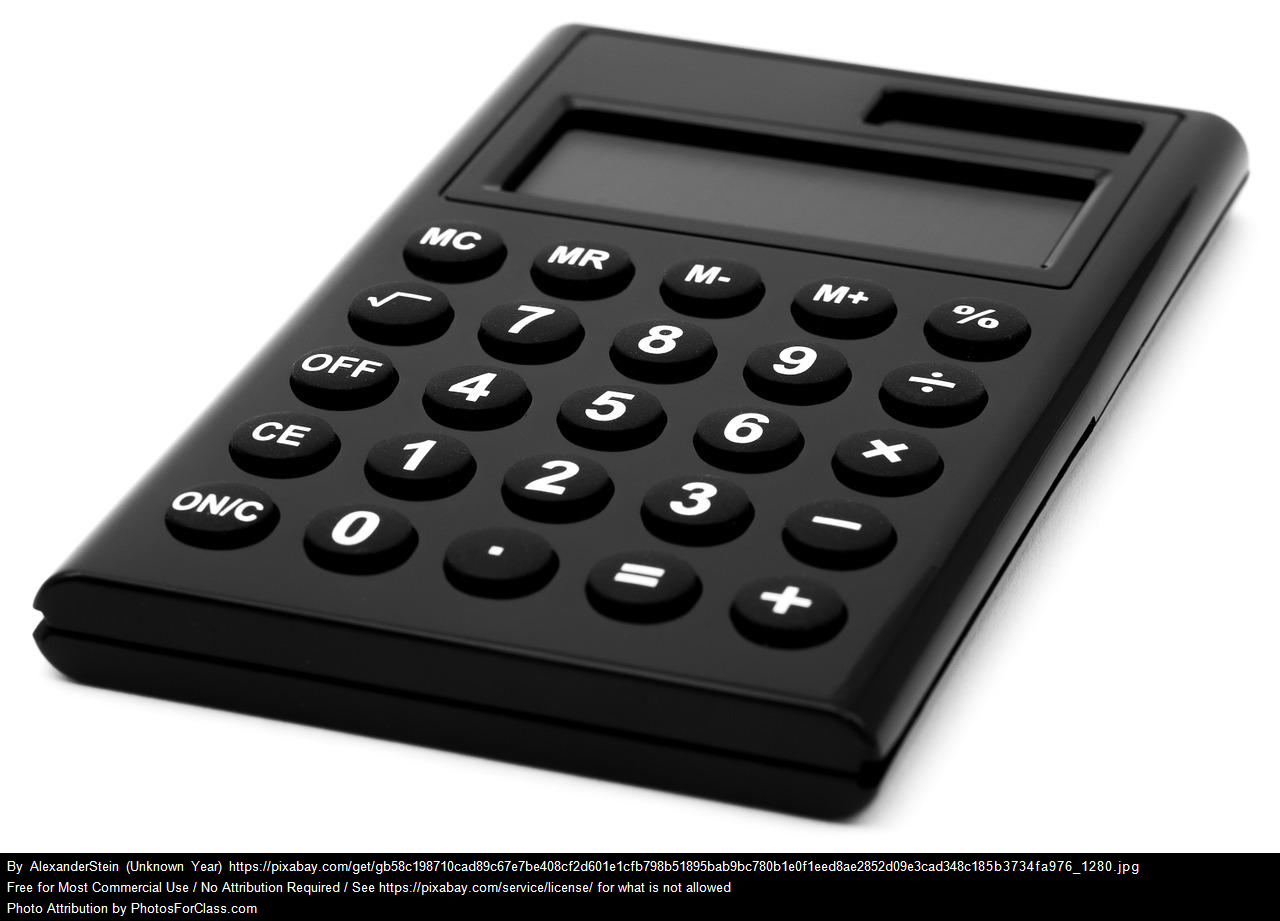
\includegraphics[scale=0.4]{Calc.png}
    \caption{Generic Calculator}
    \label{calc}
\end{figure}

\end{document}